\section{R\'esum\'e en fran\c cais}
%-----------------------------------------------------------------------------
%-----------------------------------------------------------------------------
%-----------------------------------------------------------------------------
\subsection*{Introduction}
\begin{figure}
	{\centering
		\includegraphics[width=0.95\textwidth]{graphics/ILC_scheme.jpg}
		\caption{\sl Schematic view of the ILC accelerator complex.}
		\label{fig:ILCSchemeF}
	}
\end{figure}

\begin{figure}
	\centering
	\begin{subfigure}{0.5\textwidth}
		\includegraphics[width=0.95\textwidth]{graphics/ILD.png}
		
	\end{subfigure}% 
	\begin{subfigure}{0.5\textwidth}
		\centering
		\includegraphics[width=0.9\textwidth]{graphics/ILDtracking.png}
		
	\end{subfigure}
	\caption{\sl Left: Schematic view of the ILD concept. Right: Zoom in the inner detectors.}
	\label{fig:ILDSchemeF}
\end{figure}
%-----------------------------------------------------------------------------
%-----------------------------------------------------------------------------
%-----------------------------------------------------------------------------
\subsection*{Calorim\`etre \'electromagn\'etique silicium-tungst\`ene hautement granulaire}

\begin{figure}[H]
	\centering
	\includegraphics[width=0.55\textwidth]{ECAL/graphics/ecal-new.png}
	\caption{\label{fig:ECAL-schemeF} \sl A schematic view of the \ecalp.}
\end{figure}

%-----------------------------------------------------------------------------
%-----------------------------------------------------------------------------
%-----------------------------------------------------------------------------
\subsection*{L'algorithme de reconstruction des traces}

\begin{figure}
	\centering
	\begin{subfigure}{0.5\textwidth}
		\centering
		\includegraphics[width=.90\linewidth]{ECAL/graphics/before.png}
		\caption{\label{fig:beforeF} \sl with interaction region.}
	\end{subfigure}% 
	\begin{subfigure}{0.5\textwidth}
		\centering
		\includegraphics[width=.90\linewidth]{ECAL/graphics/after2.png}
		\caption{\label{fig:afterF} \sl without interaction region.}
	\end{subfigure}
	\caption{ \sl Event display of a primary pion with an energy of 10\,GeV recorded at FNAL 2008 testbeam before \textit{(a)} and after removal of the interaction region \textit{(b)}. Smaller cubes are pads that are part of the interaction region and are not processed by the \tfa . In this event the hits in the first ten layers are classified as hits left by a primary particle.}
	%Event 16-17 in Data10.root
	\label{fig:testF}
\end{figure}


\begin{figure}
	\centering
	\includegraphics[width=0.55\textwidth]{ECAL/graphics/demo-v3.pdf}
	\caption{\label{fig:democlusterF} \sl Illustration of the clusterisation step. The \ecal\ hits are represented by blue cubes, and the search region for adjacent hits is indicated by red cubes. The blue arrows point in the direction of the clusterisation flow. }
\end{figure}

%-----------------------------------------------------------------------------
%-----------------------------------------------------------------------------
%-----------------------------------------------------------------------------

\subsection*{Comparaison des simulations avec les données réelles}



\begin{figure}
	\centering
	\begin{subfigure}{0.5\textwidth}
		\centering
		\includegraphics[width=.90\linewidth]{ECAL/plots/e-ir-2.pdf}
		\caption{\label{fig:efr2F} }
	\end{subfigure}% 
	\begin{subfigure}{0.5\textwidth}
		\centering
		\includegraphics[width=.90\linewidth]{ECAL/plots/e-ir-10.pdf}
		\caption{\label{fig:efr10F} }
	\end{subfigure}
	\caption{\label{fig:irexampleF} \sl% {\bf Fig.~\ref{fig:efr2}: Remind me how the linear plot looks like} 
		Comparison of $f_{IR}$ between data and Monte Carlo simulations for three {\sc Geant}4 physics lists for energies of 2 (a) and 10 (b) GeV of the primary particle, respectively. The first bin contains events without a detected interaction region. All histograms are normalised to unity. Error bars represent statistical uncertainties only.}
\end{figure}

\begin{figure}
	\centering
	\includegraphics[width=0.5\textwidth]{ECAL/plots/e-ir-graph.pdf}
	\caption{\label{fig:irgraphF} \sl  Mean fraction of energy deposition in the interaction region in \ecal\ for data and  Monte Carlo simulations for three {\sc Geant}4 physics lists as a function of the beam energy (2\,GeV to 10\,GeV). Events without a detected interaction region according to Sec.~\ref{sec:iazone} are discarded. The error bars represent statistical uncertainties and the error band the systematic error from the correction for double $\pi$ events.}
\end{figure}

\begin{figure}
	\centering
	\begin{subfigure}{0.5\textwidth}
		\centering
		\includegraphics[width=.90\linewidth]{ECAL/plots/r-ir-2.pdf}
		\caption{\label{fig:rir2F} }
	\end{subfigure}% 
	\begin{subfigure}{0.5\textwidth}
		\centering
		\includegraphics[width=.90\linewidth]{ECAL/plots/r-ir-10.pdf}
		\caption{\label{fig:rir10F} }
	\end{subfigure}
	\caption{\label{fig:rirexampleF} \sl %{\bf Same remark as for Fig.~\ref{fig:efr2} }
		Comparison of $r_{IR}$ distributions for data and Monte Carlo simulations for three {\sc Geant}4 physics lists for energies of the primary particle of 2 (a) and 10 (b) GeV, respectively. All histograms are normalised to unity. Error bars represent statistical uncertainties only.}
\end{figure}

\begin{figure}
	\centering
	\includegraphics[width=0.5\textwidth]{ECAL/plots/r-ir-graph.pdf}
	\caption{\label{fig:irrgraphF} \sl Mean $r_{IR}$ for data and Monte Carlo simulations for two {\sc Geant}4 physics lists as a function of the beam energy. Events without a detected interaction region according to Sec.~\ref{sec:iazone} are discarded. Error bars represent statistical uncertainties only and the error band the systematic error from the correction for double $\pi$ events.}
\end{figure}

\begin{figure}
	\centering
	\begin{subfigure}{0.5\textwidth}
		\centering
		\includegraphics[width=.90\linewidth]{ECAL/plots/ntracks-2.pdf}
		\caption{\label{fig:tr2F} }
	\end{subfigure}% 
	\begin{subfigure}{0.5\textwidth}
		\centering
		\includegraphics[width=.90\linewidth]{ECAL/plots/ntracks-10.pdf}
		\caption{\label{fig:tr10F} }
	\end{subfigure}
	\caption{\label{fig:trackexampleF} \sl Comparison of the number of secondary tracks between data Monte Carlo simulations for three {\sc Geant}4 physics lists  for energies of the primary particle of 2 (a) and 10 (b) GeV. Events without a detected interaction region according to Sec.~\ref{sec:iazone} are discarded. Error bars represent statistical errors only.}
\end{figure}

\begin{figure}
	\centering
	\begin{subfigure}{0.5\textwidth}
		\centering
		\includegraphics[width=.90\linewidth]{ECAL/plots/ntracks-graph.pdf}
		\caption{\label{fig:tracksgraphF} }
	\end{subfigure}% 
	\begin{subfigure}{0.5\textwidth}
		\centering
		\includegraphics[width=.90\linewidth]{ECAL/plots/ntracks-graph-delta.pdf}
		\caption{\label{fig:dtracksgraphF}}
	\end{subfigure}
	\caption{\label{fig:fulltrackgraphF} \sl Mean number of secondary tracks $\left<N_{tracks}\right>$ for $\varepsilon = 0.03$ (a) and the corresponding sensitivity according to Eq.~\ref{eq:sens} of $\left<N_{tracks}\right>$ on the \ep\,(b) for data and Monte Carlo simulations for three {\sc Geant}4 physics lists as a function of the beam energy (from 2 to 10\,GeV). }
\end{figure}

\begin{figure}
	\centering
	\begin{subfigure}{0.5\textwidth}
		\centering
		\includegraphics[width=.90\linewidth]{ECAL/plots/calibrationfit-2.pdf}
		\caption{\label{fig:calib2F} }
	\end{subfigure}% 
	\begin{subfigure}{0.5\textwidth}
		\centering
		\includegraphics[width=.90\linewidth]{ECAL/plots/calibrationfit-10.pdf}
		\caption{\label{fig:calib10F} }
	\end{subfigure}
	\caption{\label{fig:calibF} \sl Histograms of the energy deposition in secondary tracks for the data with 2 (a) and 10 (b) GeV beam energies. The spectra are fitted by the convolution of a Landau and a Gaussian. Events without a detected interaction region according to Sec.~\ref{sec:iazone} are discarded. Error bars represent statistical uncertainties only.}
\end{figure}

\begin{figure}
	\centering
	\includegraphics[width=0.5\textwidth]{ECAL/plots/calibrationfit-graph.pdf}
	\caption{\label{fig:calibrationgraphF} \sl MPV of the Landau fit to the $E_{dep}^t$ distributions of the pencil-like secondary tracks as a function of the beam energy for $\pi^-$ data and three Monte Carlo samples. The MPV point the of 2\,GeV data sample is excluded because of the small statistics left after selection. Events without a detected interaction region  according to Sec.~\ref{sec:iazone} are discarded.  Error bars represent the statistical fit uncertainty.}
\end{figure}

%-----------------------------------------------------------------------------
%-----------------------------------------------------------------------------
%-----------------------------------------------------------------------------

\subsection*{Les quarks top et bottom \'a l'ILC}
Electroweak production of the fermion pairs proceeds through the $f\bar{f}X$ vertex, where $X$ represents neutral vector bosons, photon or $Z^0$ boson.  The current at the $f\bar{f}X$ vertex can be expressed via form factors $F$ as 
\begin{equation}
\Gamma^{f\bar{f}X}_\mu (k^2,q,\bar{q}) = ie\{ \gamma_\mu (F^X_{1V}(k^2) + \gamma^5 F^X_{1A}(k^2)) - \frac{\sigma_{\mu\nu}(q-\bar{q})^\nu}{2m_f}(iF^X_{2V}(k^2) + \gamma^5 F^X_{2A}(k^2)) \},
\end{equation}
where $k^2= (q+\bar{q})^2$ is the four momentum squared of the exchanged vector boson, $q$ and $\bar{q}$ are the four vectors of the fermion $f$ and antifermion $\bar{f}$ and $m_f$ is the fermion mass. Further, $\gamma_\mu$ and $\gamma_5$ are the Dirac matrices, and $\sigma_{\mu\nu} = i/2(\gamma_\mu\gamma_\nu - \gamma_\nu\gamma_\mu)$.

The \sm\ values of the form factors are the following:
\begin{equation}
F^{f\gamma}_{1V} = Q^{f}, \ F^{f\gamma}_{1A} = 0, \ F^{fZ}_{1V} = \frac{I^f - 2Q^f\sin^2\theta_W}{2\cos\theta_W\sin\theta_W}, \ F^{fZ}_{1A} = - \frac{I^f}{2\cos\theta_W\sin\theta_W},
\label{formula:SMformFactors_3F}
\end{equation}
and all $F_2$ factor are zero. In the Eq.~\ref{formula:SMformFactors_3F} $I^f$ is the weak isospin number, $I^t = 1/2$ for top and $I^b = -1/2$ for bottom quark and $Q^f$ is the electric charge, $Q^t = 2/3$ and $Q^b = -1/3$.

%The form factors are related to fermion couplings with left and right-handed helicity to $Z^0$ boson:
The following definition of the left-handed and right handed $Z^0b\bar{b}$ couplings is used throughout the thesis: 
\begin{equation}
%g_L^Z = (F_{1V}^Z - F_{1A}^Z), \  g_R^Z = F_{1V}^Z + F_{1A}^Z, 
g_L^Z = I^f - Q^f\sin^2\theta_W, \  g_R^Z = -Q^f\sin^2\theta_W, 
\label{formula:EWcouplings_3F}
\end{equation}

%-----------------------------------------------------------------------------
%-----------------------------------------------------------------------------
%-----------------------------------------------------------------------------

\subsection*{Reconstruction de la charge du quark bottom}
\begin{figure}
	{\centering
		\includegraphics[width=0.55\textwidth]{ILD/plots/rec-gen-table.pdf}
		\caption{\sl Comparison of the number of reconstructed tracks $N_{gen}$ to the number of generated tracks $N_{rec}$ for a given b-jet. The number of entries is color-coded for each cell. The diagonal has 49\% of all entries and it contains the jets, which have the correctly reconstructed vertices. The b-jets below diagonal have vertices with one or more particles missed by reconstruction. The row $N_{rec} = 0$ corresponds to the b-jets with no reconstructed vertices. %Right: Same comparison, but after a cut on the b-tag$> 0.8$ and a cut on the b-hadron momentum more than 20\,GeV. The diagonal contains 55\% of the jets after the cuts.
		}
		\label{fig:Table_3F}
	}
\end{figure}

\begin{figure}
	\centering
	\begin{subfigure}{0.5\textwidth}
		\includegraphics[width=0.95\textwidth]{ILD/plots/missed-tracks.pdf}
		\caption{\label{fig:MissingTracks_cos_3F} }
	\end{subfigure}% 
	\begin{subfigure}{0.5\textwidth}
		\centering
		\includegraphics[width=0.95\textwidth]{ILD/plots/missed-momentum.pdf}
		\caption{\label{fig:MissingTracks_p_3F} }
	\end{subfigure}
	\caption{\sl Polar angle~(a) and momentum~(b) distributions of the missing prongs subdivided into different categories. This is a stacked histogram. The peak at $|\cos\theta| = 0 $ is caused by the gap between TPC endplates, the peak at  $|\cos\theta| \approx 0.8$ is caused by barrel-endcap transition in the \ecal\ and the rapid increase at $|\cos\theta| \approx 0.9$ is caused by the barrel-endcap transition in the VXD and FTD system. }
	\label{fig:MissingTracks_3F}
\end{figure}

\begin{figure}
	{\centering
		\includegraphics[width=0.95\textwidth]{ILD/plots/recovery-purity-comparison.pdf}
		\caption{\sl Comparison of the purity as function of the jet b-tag, reconstructed b-hadron momentum, $N_{rec}$ and the polar angle $|\cos\theta|$ before and after the vertex recovery algorithm.  
		}
		\label{fig:RecoveryPurityComparison_3F}
	}
\end{figure}

\begin{figure}
	{\centering
		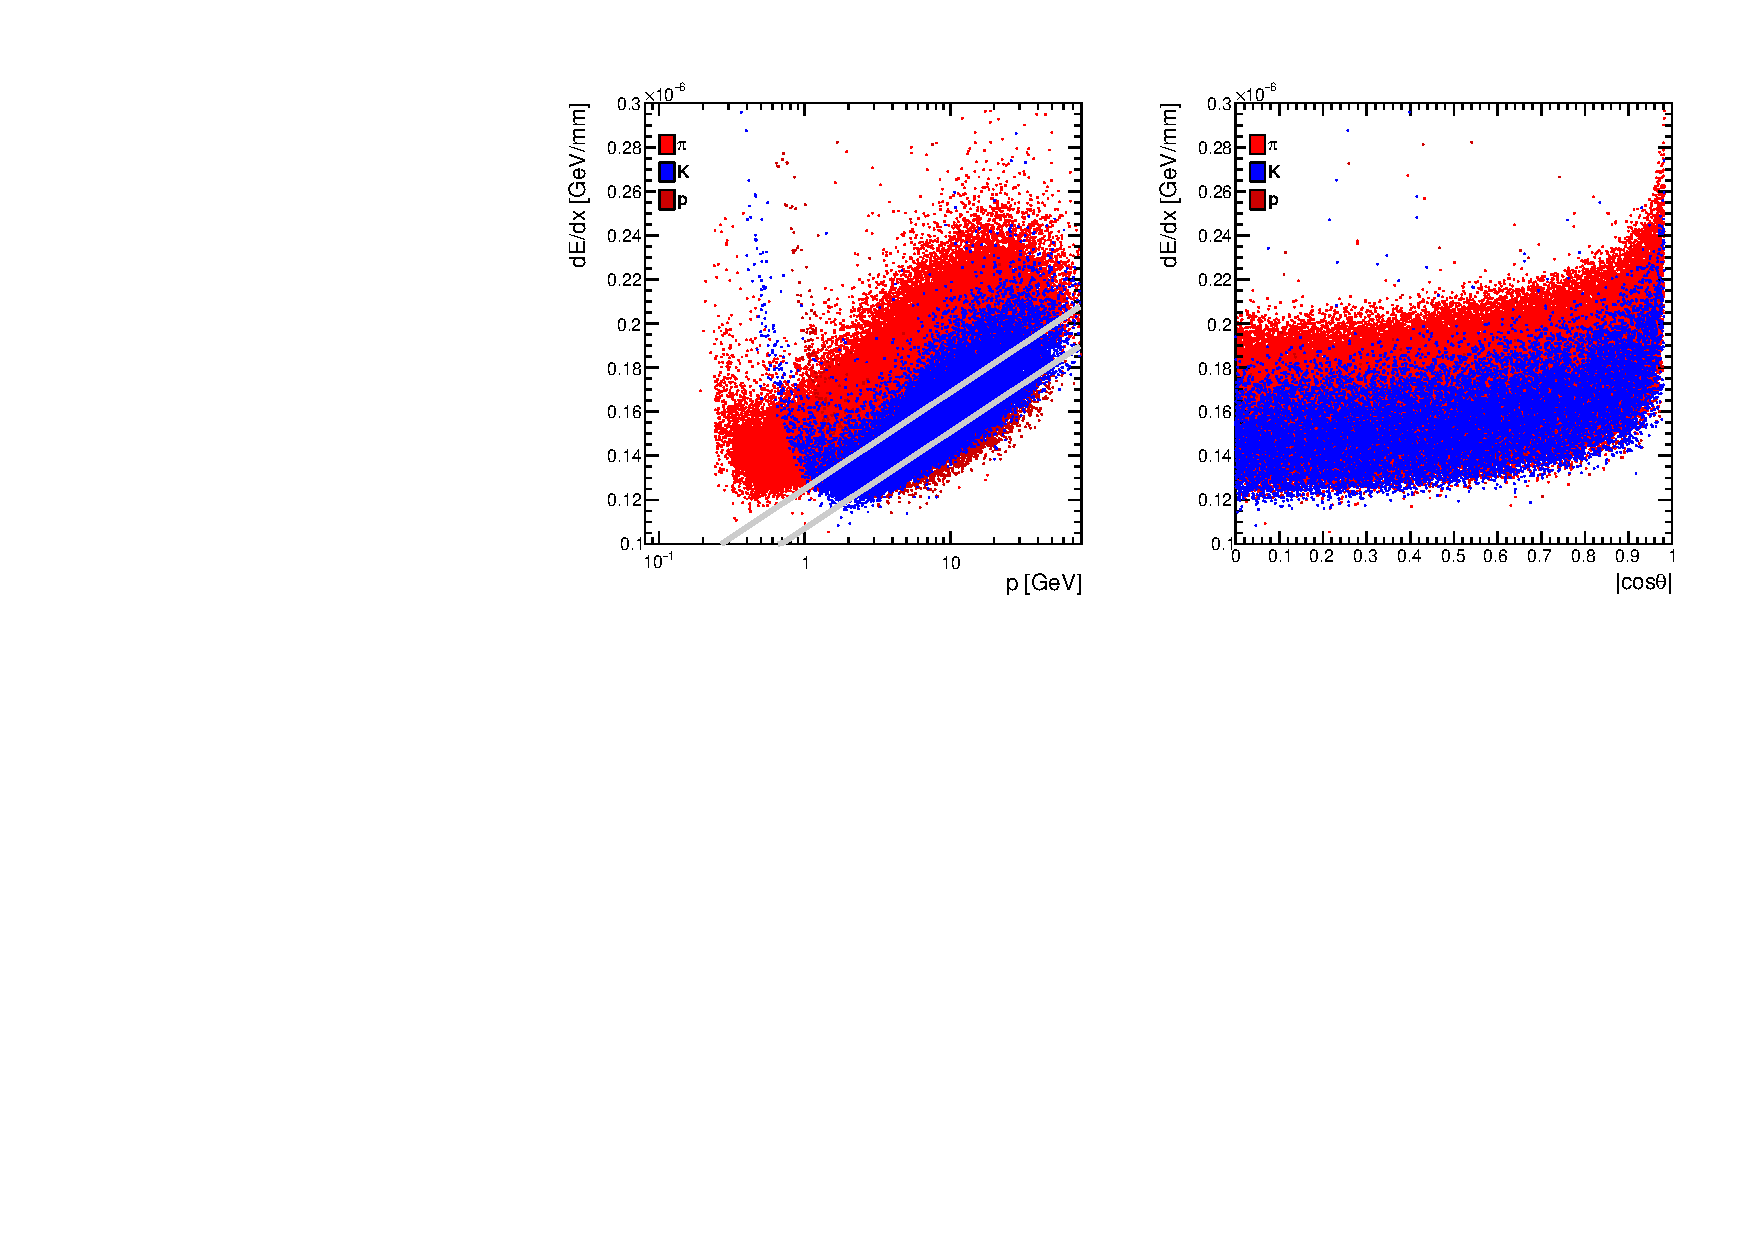
\includegraphics[clip, trim=8cm 18.5cm 7cm 4cm,width=0.95\textwidth]{ILD/plots/dedx-before.png}
		\caption{\sl The energy deposition per track length $dE/dx$ as function of the particle momentum, the particle polar angle $|\cos\theta|$ for different particles. Two gray lines separate out the region with a maximal kaon concentration. 
		}
		\label{fig:dEdxBefore_3F}
	}
\end{figure}

\begin{figure}
	{\centering
		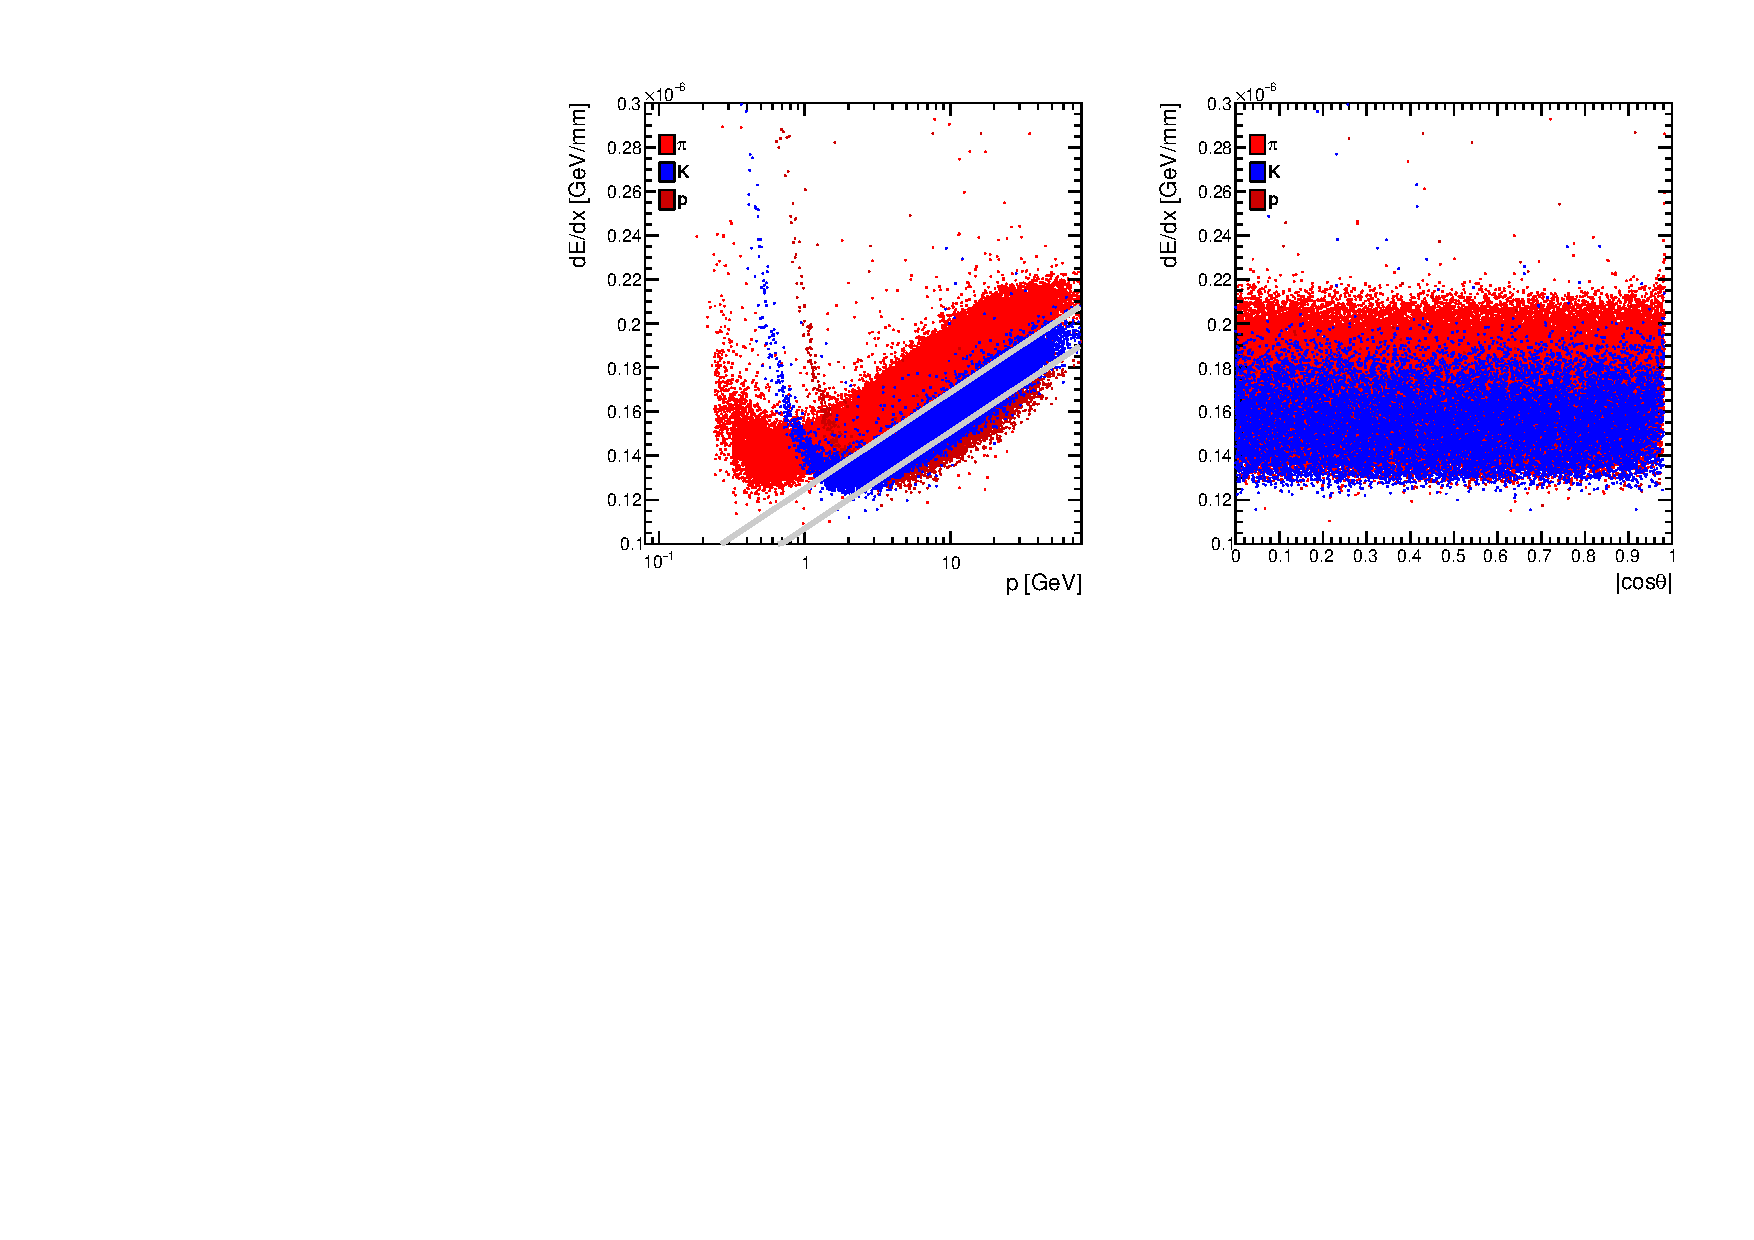
\includegraphics[clip, trim=8cm 18.5cm 7cm 4cm, width=0.95\textwidth]{ILD/plots/dedx-after.png}
		\caption{\sl The energy deposition per track length $dE/dx$ as function of the particle momentum, the particle polar angle $|\cos\theta|$ for different particles after application of the angular correction, described in text. Two gray lines separate out the region with a maximal kaon concentration. 
		}
		\label{fig:dEdxAfter_3F}
	}
\end{figure}


%-----------------------------------------------------------------------------
%-----------------------------------------------------------------------------
%-----------------------------------------------------------------------------

\subsection*{Reconstruction de l'angle polaire du quark top}


\begin{figure}
	\centering
	\begin{subfigure}{0.5\textwidth}
		\includegraphics[width=0.95\textwidth]{ILD/plots/top-asymmetry-lepton.pdf}
		\caption{\label{fig:TopAsymmetryChi_a_3F} }
	\end{subfigure}% 
	\begin{subfigure}{0.5\textwidth}
		\centering
		\includegraphics[width=0.95\textwidth]{ILD/plots/top-methods-lepton.pdf}
		\caption{\label{fig:TopAsymmetryChi_b_3F} }
	\end{subfigure}
	\caption{\sl Generated polar angle distribution compared to reconstructed polar angle (a) using all possible charge signature combinations, plotted in (b). }
	\label{fig:TopAsymmetryChi_3F}
\end{figure}

%-----------------------------------------------------------------------------
%-----------------------------------------------------------------------------
%-----------------------------------------------------------------------------

\subsection*{Reconstruction de l'angle polaire du quark bottom}

\begin{figure}
	\centering
	\begin{subfigure}{0.5\textwidth}
		\includegraphics[width=0.95\textwidth]{ILD/plots/basymmetry-final-left.pdf}
		\llap{\shortstack{%
				\includegraphics[clip, trim=0cm 0cm 1.8cm 1.7cm, scale=.14]{ILD/plots/zoom-final.pdf}\\
				\rule{0ex}{0.38in}%
			}
			\rule{1.8in}{0ex}}
		\caption{\label{fig:BAsymmetryFinal_a_3F} }
	\end{subfigure}% 
	\begin{subfigure}{0.5\textwidth}
		\centering
		\includegraphics[width=0.95\textwidth]{ILD/plots/basymmetry-final-right.pdf}
		\caption{\label{fig:BAsymmetryFinal_b_3F} }
	\end{subfigure}
	\caption{\sl Generated b-quark polar angle distribution compared to the final reconstructed b-quarks polar angle in left-handed case (a) and right-handed case (b) with overlaid background processes.  }
	\label{fig:BAsymmetryFinal_3F}
\end{figure}



\begin{figure}
	\centering
	\begin{subfigure}{0.5\textwidth}
		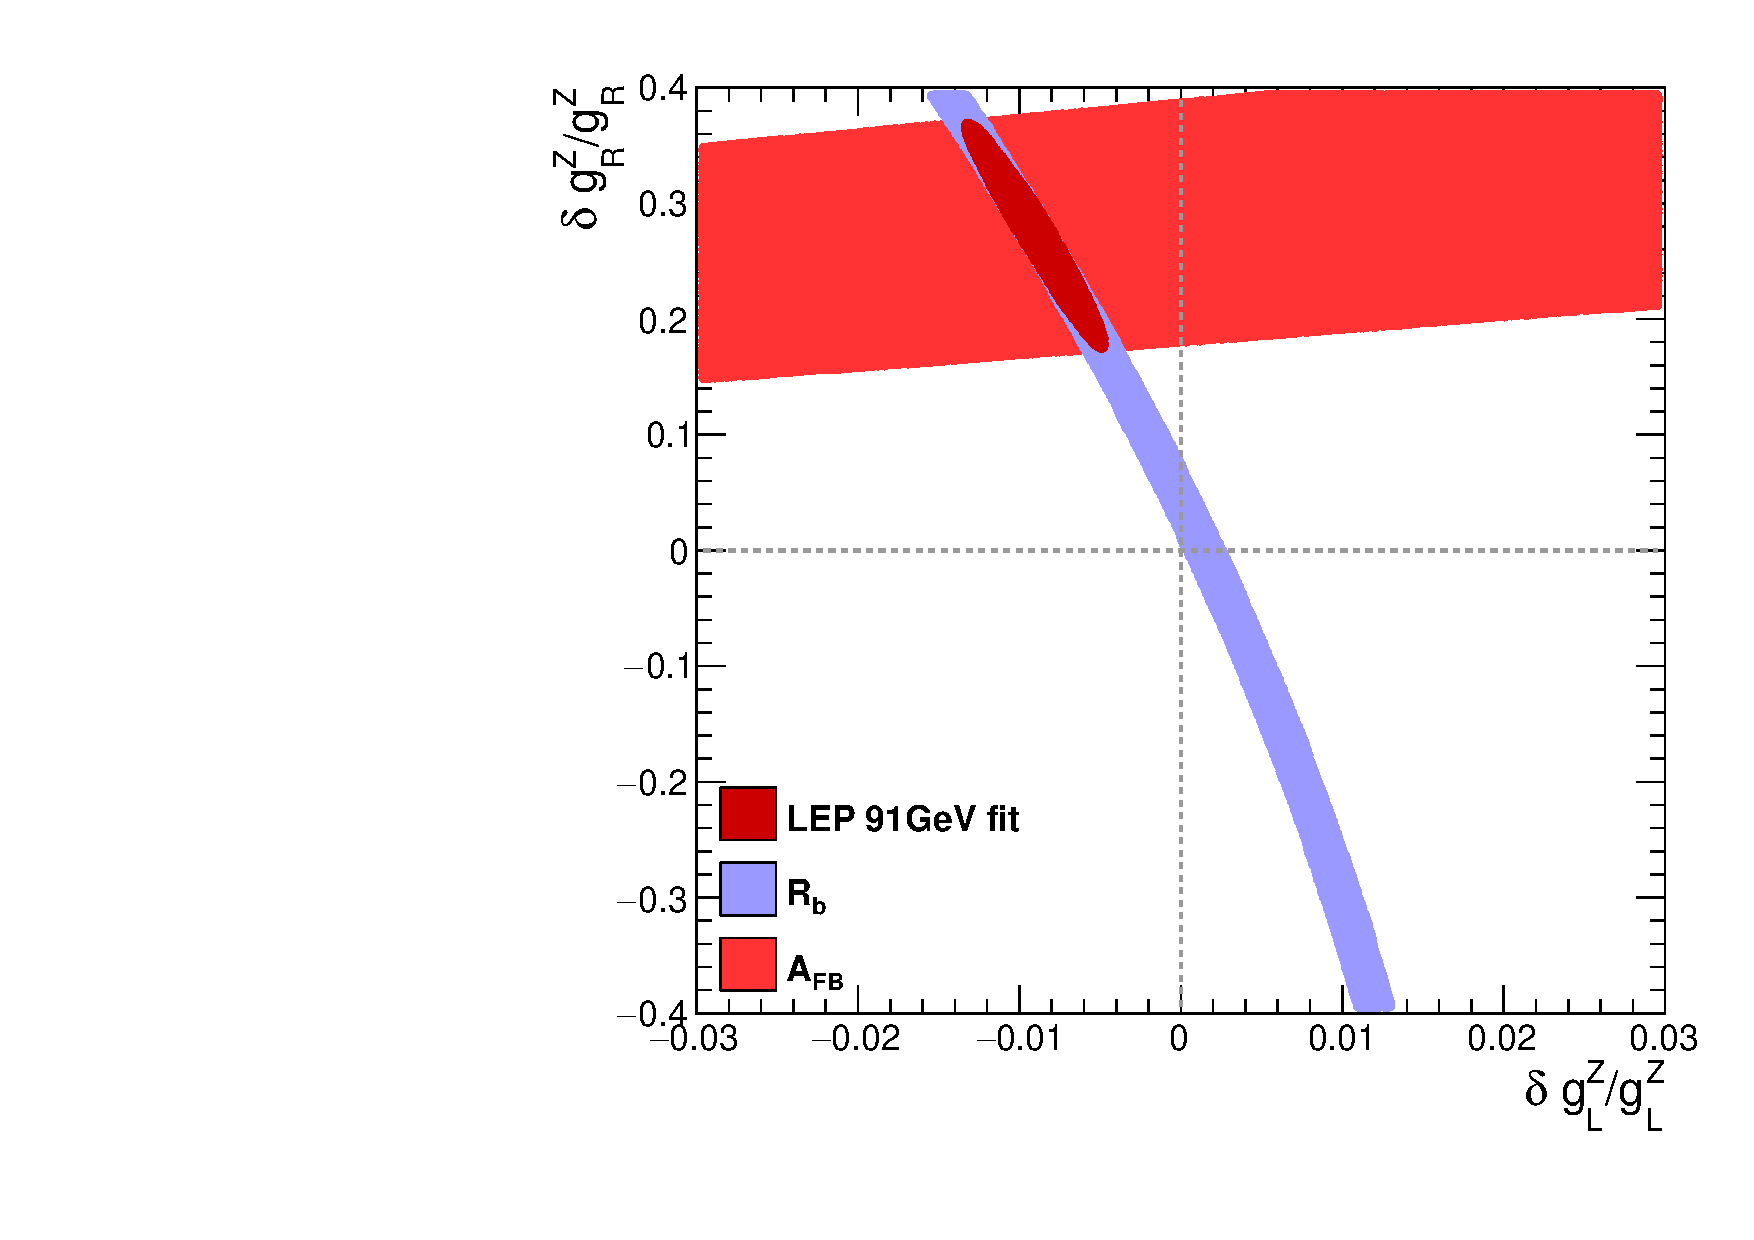
\includegraphics[width=0.99\textwidth]{ILD/plots/lep-result-zoom.pdf}
		\caption{\label{fig:LEPILCResult_a_3F} }
	\end{subfigure}% 
	\begin{subfigure}{0.5\textwidth}
		\centering
		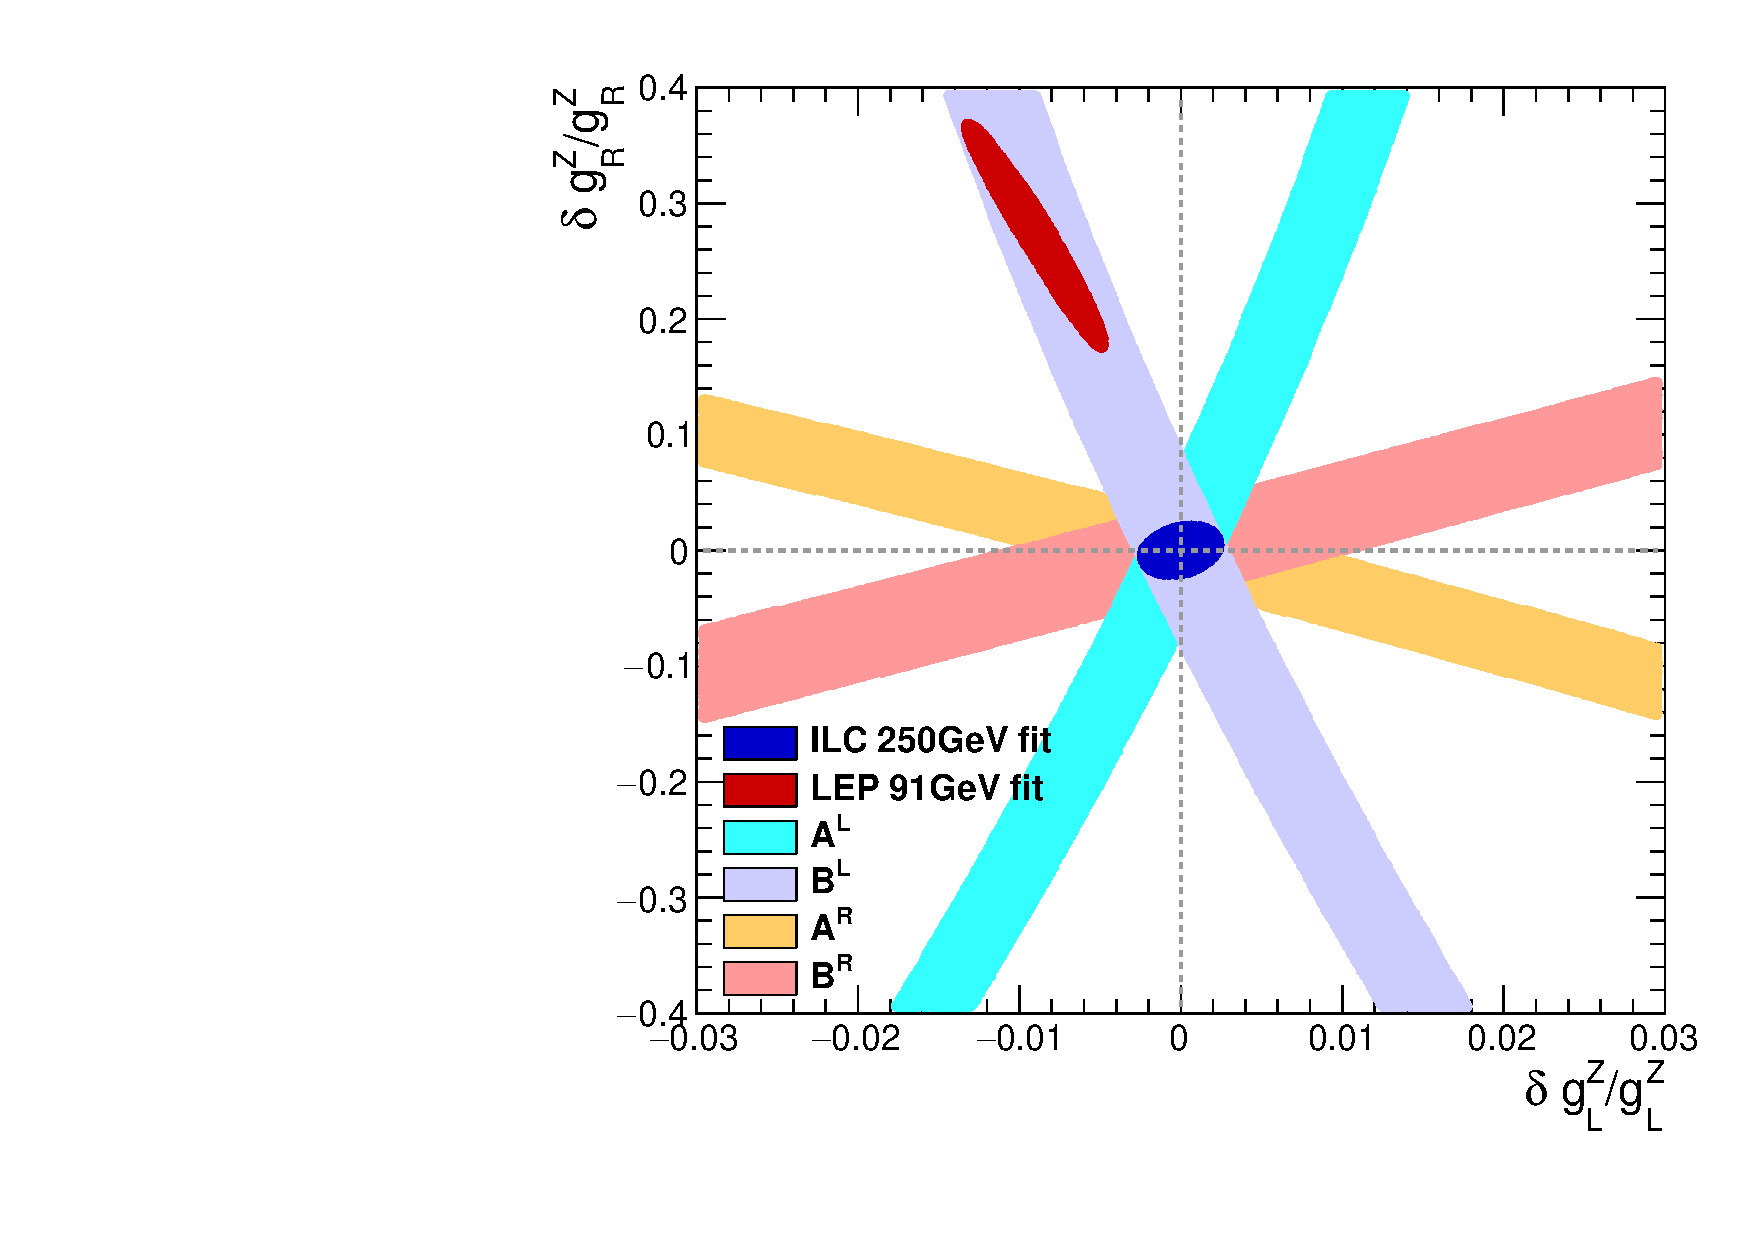
\includegraphics[width=0.99\textwidth]{ILD/plots/ilc-result.pdf}
		\caption{\label{fig:LEPILCResult_b_3F} }
	\end{subfigure}
	\caption{\sl Tree level $\pm 1\,\sigma$ allowed regions defined by the forward-backward asymmetry and total cross section measurements at LEP (a) and ILC via the differential cross section fit (b). Dashed guidelines show the \sm\ value. The allowed region expected at the ILC is centered at the \sm\ values of couplings.}
	\label{fig:LEPILCResult_3F}
\end{figure}







